\documentclass[a4paper]{article}

%% Language and font encodings
\usepackage[english]{babel}
\usepackage[utf8x]{inputenc}

\usepackage[T1]{fontenc}
\usepackage{wrapfig, blindtext}

%% Sets page size and margins
\usepackage[a4paper,top=3cm,bottom=2cm,left=3cm,right=3cm,marginparwidth=1.75cm]{geometry}

%% Useful packages
\usepackage{amsmath}
\usepackage{graphicx}
\usepackage[colorinlistoftodos]{todonotes}
%Color a las referencias
\usepackage[colorlinks=true, allcolors=blue]{hyperref}
%Color a los textos

%Caratula
\begin{document}
\begin{titlepage}
\begin{center}
\vspace*{-0.4in}

{\fontsize{12}{30}\bf \selectfont UNIVERSIDAD NACIONAL DE INGENIERIA\\}

{\fontsize{12}{40}\bf \selectfont FACULTAD DE CIENCIAS\\}
\vspace*{0.15in} CIENCIAS DE LA COMPUTACI\'ON\\
\vspace*{0.2in}


\begin{center}

\includegraphics[width=5.5cm,height=6.5cm]{UNI.png}
\end{center}
\vspace*{0.2in}

\begin{large}
	{\bf PROYECTO DE BIOLOGIA COMPUTACIONAL\\}
	\vspace*{0.3in}
\end{large}

\begin{large}
{\bf T\'itulo del Trabajo\\}
\vspace*{0.2in}
\end{large}

\begin{Large}
\color{blue}
\textbf{PhyloZofia\\}
\color{black}
\end{Large}
\vspace*{0.2in}

\begin{large}
{\bf Autores} 
\vspace*{0.1in}
\\L\'azaro Camasca, Edson Nicks\\
Leon Rios, Marco Naro
\end{large}
\vspace*{0.4in}


\begin{large}
{\bf Profesor} 
\vspace*{0.1in}
\\Nuñez Iturri, Ciro Javier
\end{large}

\end{center}
\begin{center}
\begin{large}
\vspace*{1.0in}
Lima - Peru\\
{\bf (2019)}
\end{large}
\end{center}
\end{titlepage}

\pagebreak
\tableofcontents
\pagebreak

\section{Objetivos}

\subsection{Objetivos Generales}
\begin{itemize}
\item Creación de un aplicación gráfica usando BioPython y TKinter para el analisis de información Genética de Especies endémicas de las regiones del Perú.

\end{itemize}

\subsection{Objetivos Específicos}

\begin{itemize}
\item Recolectar información genética de especies endémicas.
\item Desarrollar la aplicación para el análisis de secuencias,.
\item Desarrollar algoritmos para obtener las alineaciones, árboles filogenéticos 
\item Evaluar el árbol filogenético
\end{itemize}

\section{Resumen Ejecutivo}

Se pretender crear una aplicación gráfica conectada a una base de datos con la información genética de las especies endémicas del Perú, el software procesara las secuencias, creará el árbol filogenético, mostrará los resultados y analizará las relaciones evolutivas de las especies escogidas.
Se escogió como marcaadores moleculares a la proteína NADH deshidrogenasa subunidad 2 debido la importante función respiratoria mitocondrial, hecho por el cual tiene presencia en todas las especies escogidas.
Se realizó el alineamiento utilizando la herramienta en linea EMBL-EBI.
Se utilizó el modelo evolutivo Kimura y el método para la construcción de árbol escogido fue un método basado en agrupamiento.
Se implementó el UPGMA y el método Unión de vecinos.

\section{Descripción del Proyecto}

El proyecto sera implementado netamente en el lenguaje Python
Las librerías utilizadas serán:
\begin{itemize}
\item BioPython para el procesamiento de secuencias
\item Tkinter para el entorno gráfico.
\end{itemize}
Dentro de la GUI, se pobre escoger Especies para el análisis posterior.\\
Los datos recolectados serán reales de la base de datos de NCBI.\\
Se implementara algoritmos para el alineamiento de Genes homólogos.\\
Se implementara algoritmos para el alineamiento de Proteínas.\\
Se implementara la algoritmos para la Generación de Arboles Filogenéticos de acuerdo a un modelo.\\

\noindent Para el desarrollo del proyecto se seguirá la siguiente metodología:

\subsection{Determinar las especies y el material a utilizar}

Las especies se escogieron por ser especies endémicas del Perú, especias en \textbf{peligro de extinción} en el Perú y \textbf{especies representativas} del Perú. Además, se tuvo en cuenta la disponibilidad de material genético puesto que muchas de las especies endémicas poseen una base de datos genética incompleta y algunas no se encuentran codificadas en absoluto.\\

\noindent El material genetico se encuentran en la base de datos de NCBI, se los nombres son un enlace para poder optener más información en NCBI.\\

\noindent Se escogió las siguientes 11 especies:
\begin{itemize}
    \item \href{https://www.ncbi.nlm.nih.gov/protein/ABM63279.1/}{\underline{Tremarctos ornatus}}
    
    \item 
    \href{https://www.ncbi.nlm.nih.gov/protein/AIY56286.1}{\underline{Panthera onca}}
    
    \item 
    \href{https://www.ncbi.nlm.nih.gov/protein/ACJ45788.1}{\underline{Vicugna vicugna}}
    
    \item 
    \href{https://www.ncbi.nlm.nih.gov/protein/329756060}{\underline{Aulacorhynchus huallagae}}
    
    \item 
    \href{https://www.ncbi.nlm.nih.gov/protein/YP_009178568.1}{\underline{Leopardus jacobita}}
    
    \item 
    \href{https://www.ncbi.nlm.nih.gov/protein/NP_944712.1}{\underline{Inia geoffrensis}}
    
    \item 
    \href{https://www.ncbi.nlm.nih.gov/protein/AON77377.1}{\underline{Spheniscus humboldti}}
    
    \item 
    \href{https://www.ncbi.nlm.nih.gov/protein/AEH42425.1}{\underline{Vultur gryphus}}
    
    \item 
    \href{https://www.ncbi.nlm.nih.gov/protein/BAH23368.1}{\underline{Lama glama}}
    
    \item 
    \href{https://www.ncbi.nlm.nih.gov/protein/AJE26518.1}{\underline{Cavia porcellus}}
    
    \item 
    \href{https://www.ncbi.nlm.nih.gov/protein/298371651}{\underline{Platalea ajaja}}
    
\end{itemize}


\subsection{Elegir los marcadores moleculares}
La elección de los marcadores moleculares es una parte importante porque puede hacer una \textbf{gran diferencia} en la
obtención de un árbol correcto.

\noindent Entre los marcadores moleculares, secuencias de nucleótidos o de proteínas, se optó por utilizar \textbf{secuencias de proteínas} por las siguientes razones:


\begin{itemize}
	\item Como se va estudiar la evolución de grupos de \textbf{organismos ampliamente divergentes} se aconseja utilizar secuencias de proteínas.
	\item Las relaciones filogenéticas que se están analizando están en el \textbf{nivel más profundo - bacteriana}, por ello lo más adecuado es usar secuencias de proteínas conservadas.
\end{itemize}


\subsubsection*{Proteina NADH deshidrogenasa}

La proteína a analizarse sera el NADH deshidrogenasa, también conocido como Complejo I, subunidad 2 debido a que se encuentra presente en todas las especias y está codificado. \\
La proteína escogida cumple una importante \textbf{función en la respiración bacteriana y mitocondrial}. Por ende, es posible encontrarla en diversas especies y no es extraño que se haya codificado.\\
Una importante observación es que no todas las especies se encuentran codificadas en la base de datos de NCBI, faltando genes importantes.

\begin{center}
	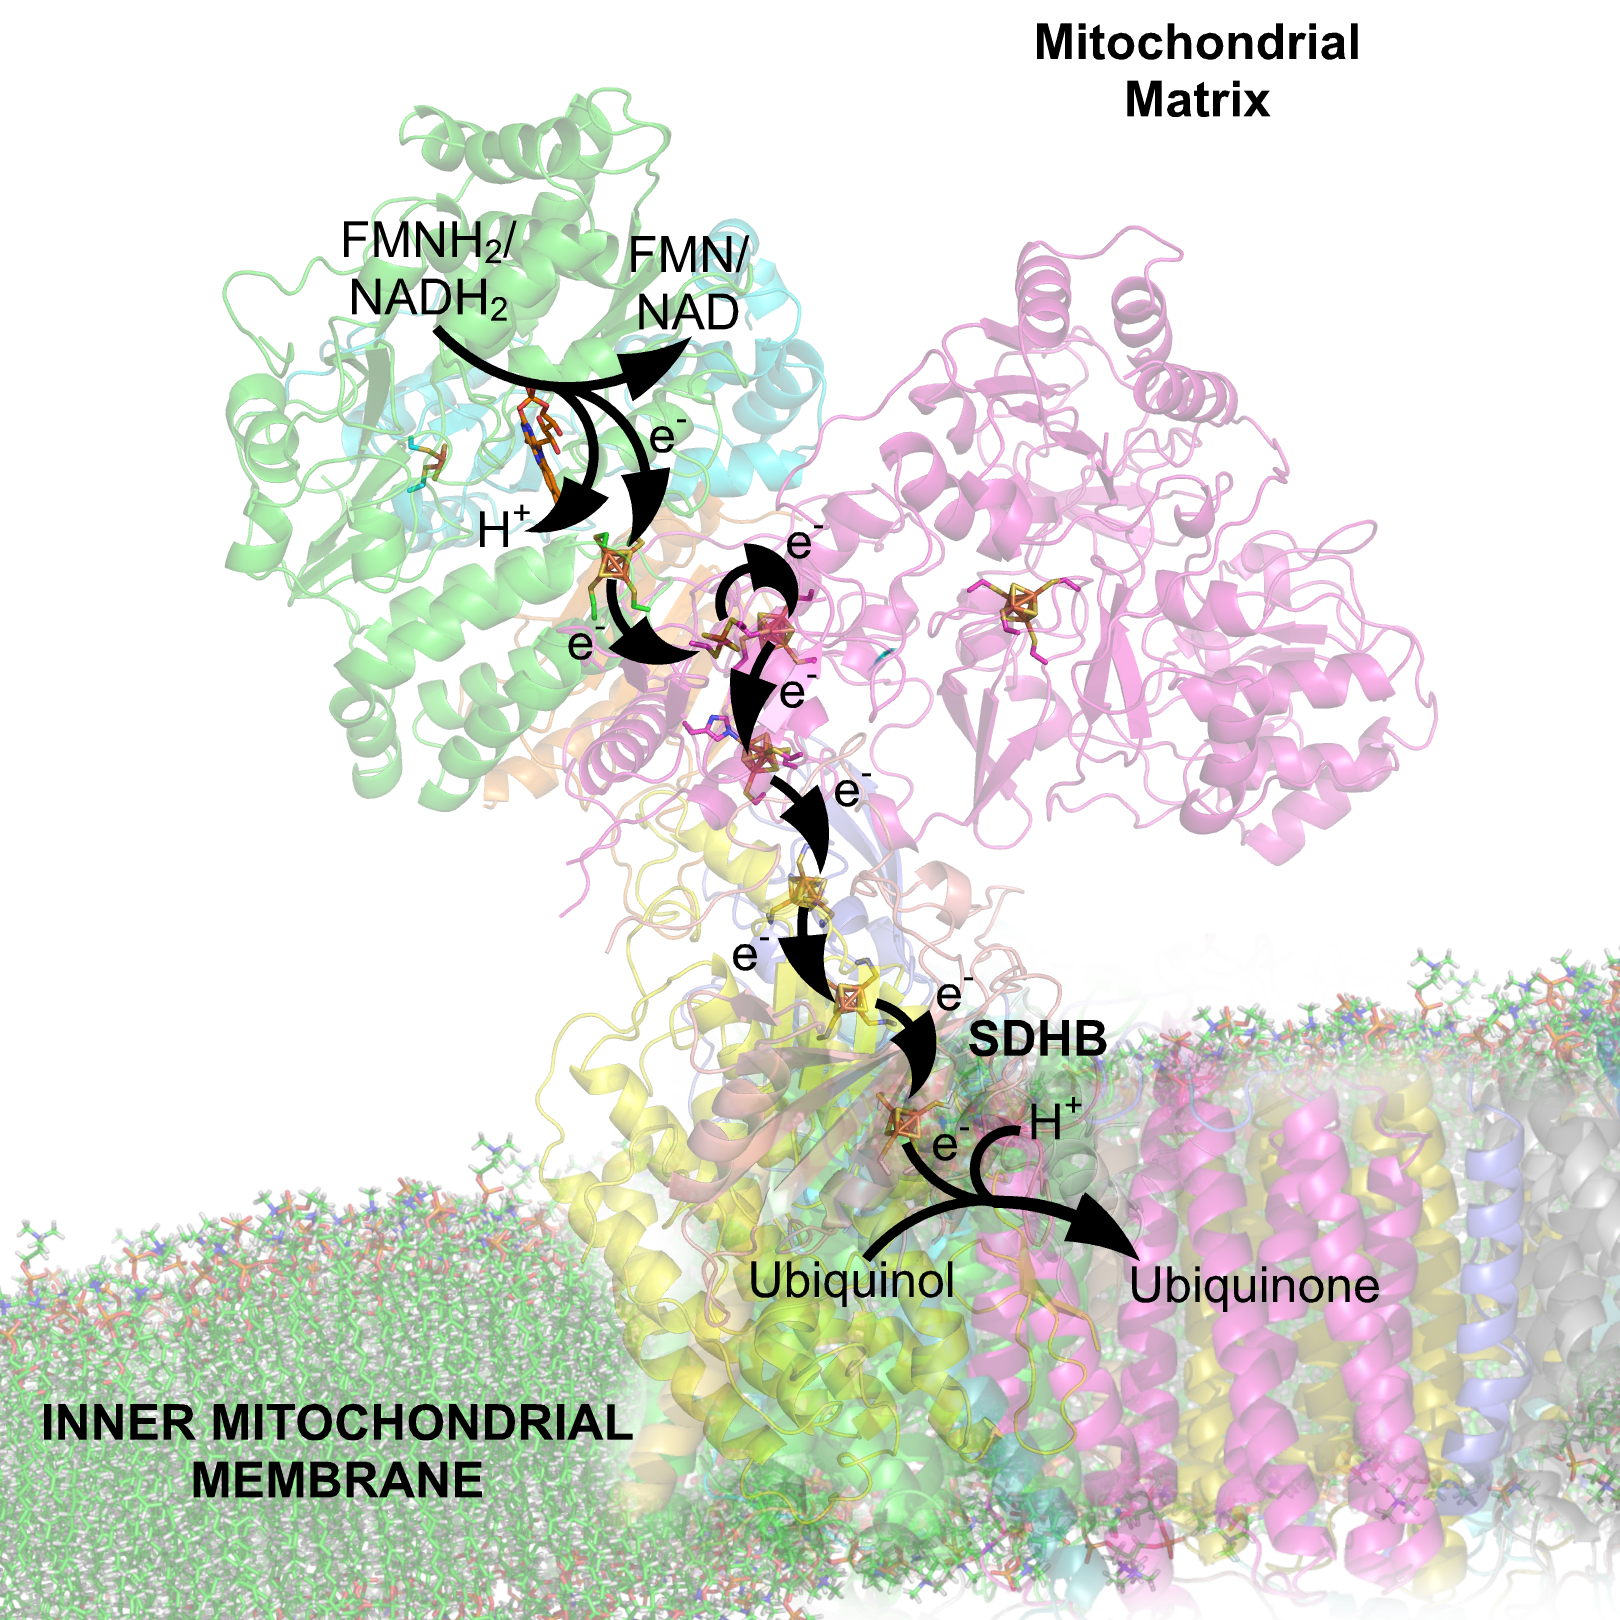
\includegraphics[width=8.5cm,height=8.5cm]{NADH.png}
	
	Fig. Proteina NADH deshidrogenasa
\end{center}


\subsection{Realizar el alineamiento múltiple de genes homólogos}
Este paso es el mas importante de todas, ya que éste establece las correspondencias posicionales en la evolución.\\
Sólo el alineamiento correcto produce inferencias filogenéticas
correctas.
\subsubsection*{EMBL-EBI}
Para la alineación de secuencias se utilizada la Web de EMBL-EBI: \textbf{Multiple Sequence Alignment} 
\href{https://www.ebi.ac.uk/Tools/msa/muscle/}{\underline{click aquí para consultar la pagina}}
\\
Las secuencias se enviaran a la Web, esta realizara la alineación luego se descargara los resultados en formato clustal.
\\
Cuando descargamos el archivo tiene el siguiente formato ".clwstrict" luego cambiamos a ".clustal".

\subsubsection*{Clustalo}
Para usuarios de Ubunto se utilizara el software de clustal.

\subsection{Modelo Evolutivo Kimura}
Ya que se quiere resultados lo más sofisticado (realista) se optara por el \textbf{Modelo Kimura}.
Este modelo considera \textbf{diferentes las tasas de mutación} para las transiciones (substitución de una purina por otra o una pirimidinas por otra) y para las transversiones (substitución de una purina por una pirimidina o vice versa)\\

De acuerdo a este modelo las transiciones ocurren más frecuentemente que las transversiones, lo cual provee mejores estimaciones de la distancia evolutiva


\subsubsection{Construcción de la matriz de distancias}
A partir del modelo Kimura tenemos:\\

$d_{AB} = −(1/2) ln(1 − 2p_{ti} − p_{tv}) − (1/4) ln(1 − 2p_{tv})$\\

\noindent Donde:\\
$p_{ti}$ es la frecuencia observada de transición.\\
$p_{tv}$ es la frecuencia de transversión.\\

\noindent Las distancias evolutivas calculadas pueden ser usadas para
construir una matriz de distancias entre todos los pares de taxones

\subsection{Métodos para la construcción de árbol filogenético}	

Los algoritmos basados en distancias para construir árboles
filogenéticos pueden ser subdivididos:

\subsubsection*{Métodos basados en agrupamiento}

Los algoritmos basados en agrupamiento calculan el árbol
usando una matriz de distancias e iniciando por los pares de
secuencias más similares.

\noindent Un gran ventaja es la habilidad para hacer uso de \textbf{diferentes modelos de substitución} para corregir las distancias evolutivas.

\subsubsection*{Métodos basados en optimalidad}

Los algoritmos basados en optimalidad comparan muchas
topologías alternativas de árboles y seleccionan el que tenga el
mejor ajuste entre las distancias estimadas en el árbol y las
distancias evolutivas reales

\noindent Los metodos basados en optimalidad requieren \textbf{mucha capacidad de computo} debido a la búsqueda exhaustiva que realizan, por ello se optó por escoger basados en agrupamiento.

\noindent El usuario podra escoger dos metodos, a partir de la interfaz grafica:
\subsubsection{UPGMA}
UPGMA (unweighted pair group method using arithmetic average)
El método más simple basado en agrupamiento.

\subsubsection{Unión de Vecinos}
El método de "Unión de vecinos" parte de una matriz de distancias, que indica la distancia entre cada par de taxones. El algoritmo comienza con un árbol completamente sin resolver, cuya topología corresponde a la de una red en estrella, y aplica los siguientes pasos hasta que el árbol está completamente resuelto y las longitudes de sus ramas.\\

\noindent Ahora que ya sabemos los pasos para la creación de arboles filogeneticos pasamos a la implementación.


\section{Algoritmos e implementación computacional}
\textbf{Una descripción de los algoritmos y herramientas que se [planean utilizar en caso de la propuesta] utilizados incluyendo pseudo código y código fuente}\\
\subsection{Prerrequisitos}

Los prerrequisitos para repliacar el proyecto son:
\subsubsection*{Python}
Instalar python desde \href{https://www.python.org/downloads/}{\underline{Python}} para windows o 'sudo apt-get install python3.6' para linux.
\subsubsection*{BioPython}
BioPython es un paquete Python muy popular para manejar información biologica.
Para instalar:

conda install biopython
ó
pip install biopython

BioPython tiene tres funcionalidades principales:
Sequence Handling, 3D Structure, Population Genetics.


\noindent Antes de pasar con la implemetacion necesitamos saber con que tipo de datos vamos a trabajar, estos datos se encuentran en  archivos con terminación fasta, xml, clustal, etc. Para establecer un orden y facilidad el mantenimiento de los algoritmos estos se encontraran en una carpeta \textbf{data-gen}.

\subsection{Obtener Secuencias}
\noindent Si usted quiere replicar el proyecto con otras especies, lo unico que tiene que hacer es descargar sus secuencias en formato .fasta de NCBI y agregarlas al directorio data-gen/fasta, ver la siguiente imagen.

\begin{center}
	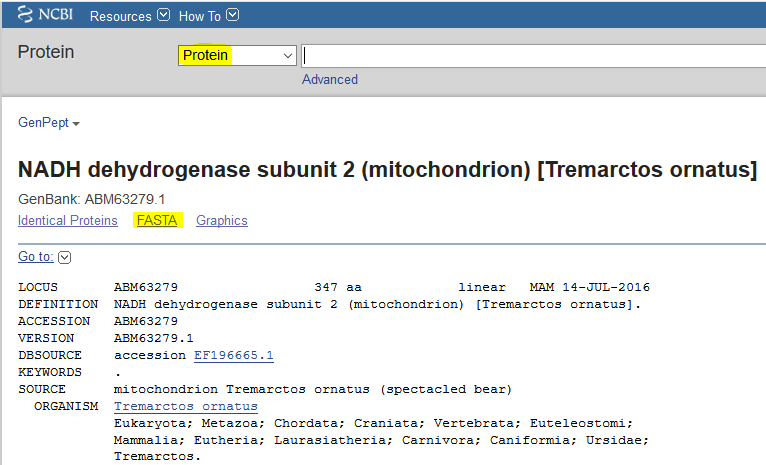
\includegraphics[width=12.5cm,height=8.5cm]{ncbi_replica.png}
	
	Fig. Descargar la secuencia .fasta haciendo click en \underline{FASTA}
\end{center}

\noindent BioPython ya tienen implementado algunos algoritmo para el manejo y alineamiento de secuencias, creacion de arboles estos nos facilitan el trabajo, ya no se tiene que inventar la rueda.

\subsection{Union de archivos fasta}

Una vez que tenemos todos nuestros archivos .fasta, pasamos a seleccionar aquellos organismos que nos interasan para su posterior análisis.

\noindent Para la selección hacemos uso de una lista llamada elegidos = [  ] que contenca los indices de las secuencias elegidas. Creamos una funcion que reciba la lista elegidos y crea un archivo en data-gen llamado \textbf{Sec-Unidas.fasta}.

\begin{center}
	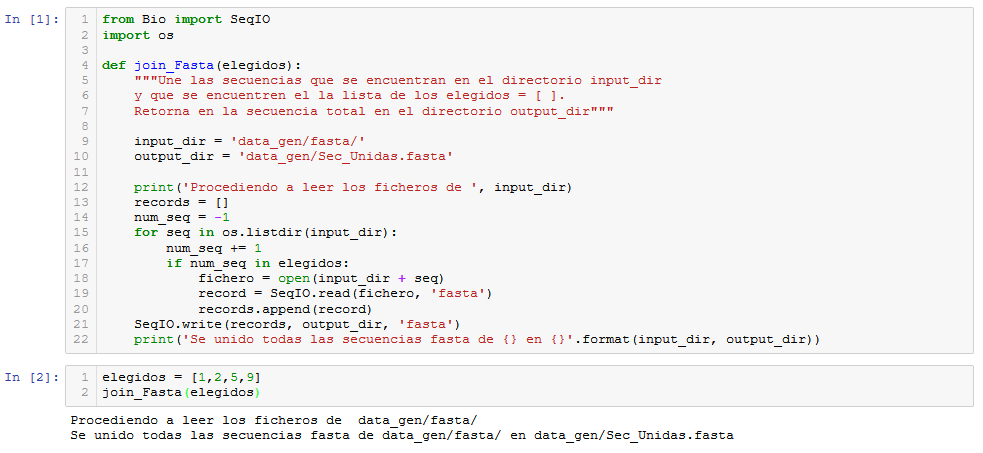
\includegraphics[width=16cm,height=9cm]{join_Fasta.png}
\end{center}

Ahora que tenemos las secuencias unidas en un solo archivo pasamos a alinearlas.

\subsection{Alineamiento de Secuencias}

\noindent Al alinear dos o más secuencias podemos observar las partes donde ellas difieren e inferir información útil sobre ellas

\noindent Un tipo de información útil es la filogenia. Esto implica que podemos inferir cómo la evolución puede explicar un conjunto particular de secuencias observadas

Para el alineamiento se utilizara la herramienta \href{http://www.clustal.org/}{\underline{Clustal}} este nos proporciona el alineamiento tanto para Windows como para Linux.

\subsubsection{Alineamiento en Windows}
Si estamos usando windows usamos \href{http://www.clustal.org/omega/}{\underline{Clustal Omega}}, una vez descargado el programa podemos hacer uso de este revisando el archivo README que viene con el programa.
  
\noindent El algoritmo para la implementacion recibe el archivo de las secuencias unidas y genera un archivo \textbf{.clustal} con el alineamiento, se hace uso de comandos de sistema. \\

 
\begin{center}
	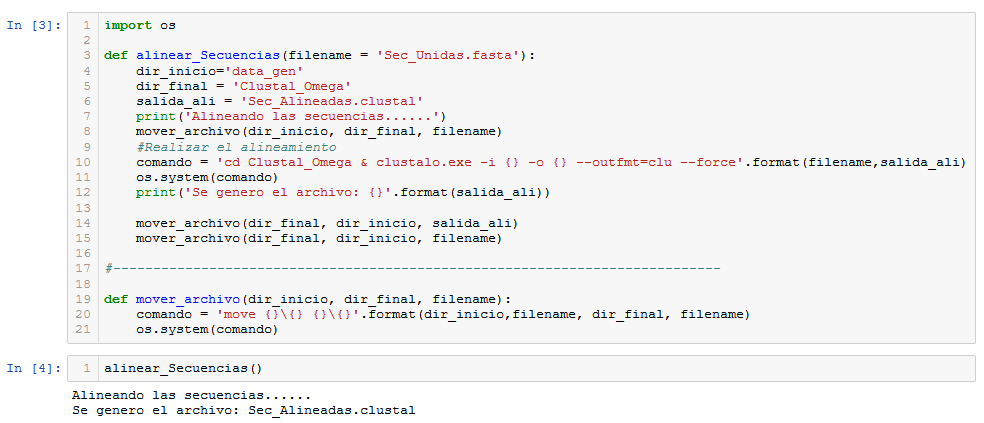
\includegraphics[width=16cm,height=7cm]{Alin_Sec.png}
\end{center}

\subsection{Lectura de Secuencias Alineadas}
Para poder hacer uso de las secuencias alineadas tenemos que almacenarla en una variable o tambien llamado objeto alineamiento. El siguiente algoritmo recibe la direccion del archivo clusta y retorna el objeto aligment.

\begin{center}
	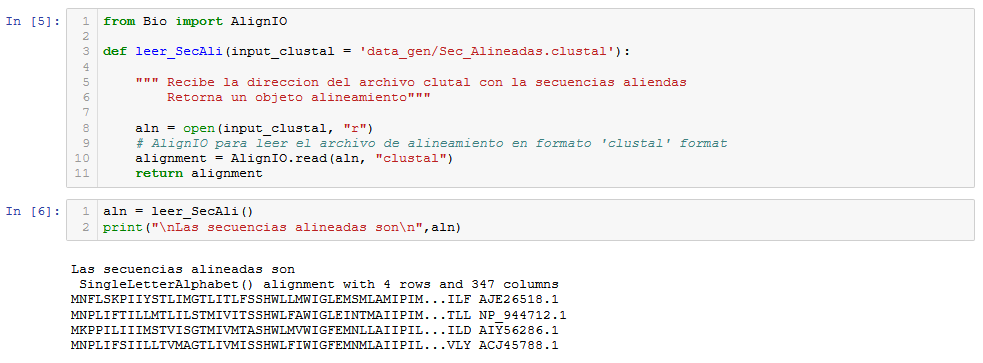
\includegraphics[width=16cm,height=7cm]{leerAlin.png}
\end{center}


\subsection{Creación de la Matriz de Distancias}
Usando el parsing del alienamiento , podemos obtener la distancia (o diferencia) entre todas las secuencias.

Esto nos indica, para cada par de secuencias, cuan diferentes son.
Para el caso ejemplo usamos como parametro 'identity', tambien esta el parametro 'blosum62' que toma diferentes valores de transición y transversión. 
\begin{center}
	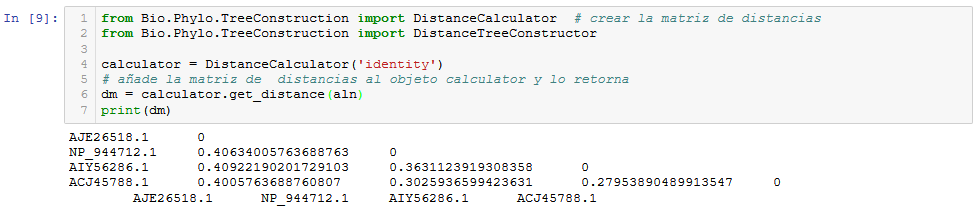
\includegraphics[width=16cm,height=5cm]{matriz.png}
\end{center}

\subsection{Creación del Arbol Filogenetico}
Finalmente, podemos construir un arbol filogenético a partir de las distancias entre todas las secuencias.
Se crea una función donde se pueda escoger el tipo de arbol a crear entre el upgma y nj(union de vecinos).

\begin{center}
	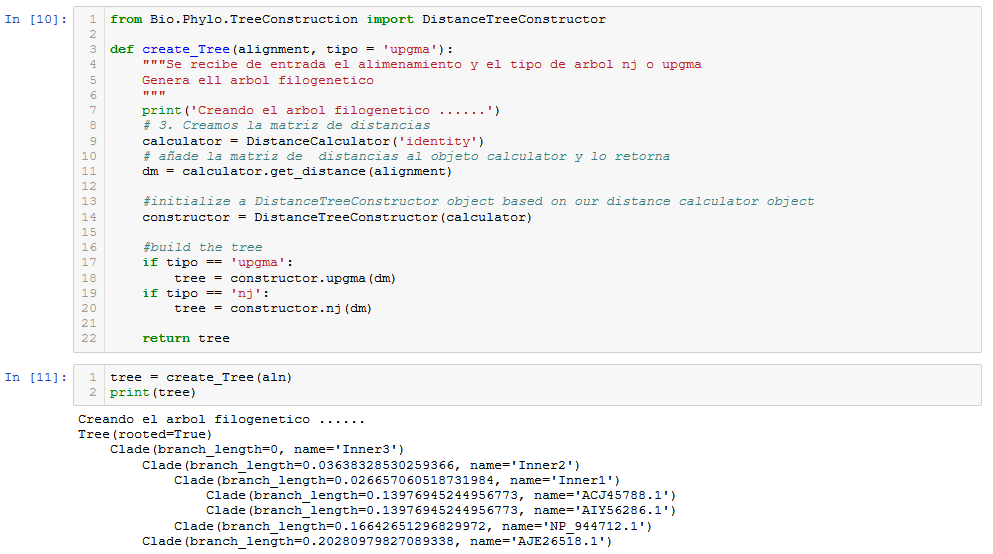
\includegraphics[width=16cm,height=10cm]{CrearArbol.png}
\end{center}
Una vez creado el objeto arbol pasamos mostrar el arbol

\subsubsection*{Mostrar Arbol}
Para mostrar el arbol usamos la funcion \textbf{Phylo.draw()}, a partir de este arbol se puede realizar el análisis.
 
\noindent 
\begin{center}
	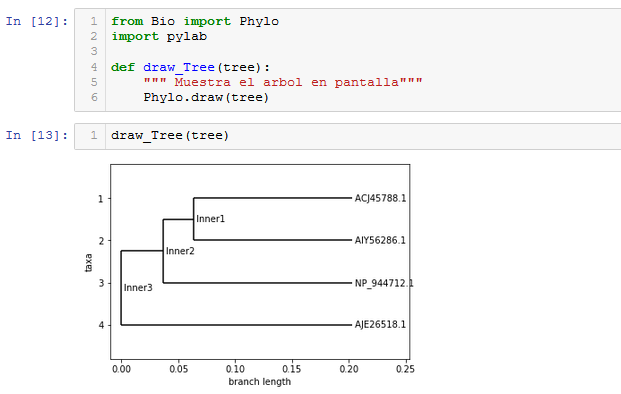
\includegraphics[width=11cm,height=5cm]{mostrarArbol.png}
\end{center}

\subsection{Interfaz Grafica}
\noindent Todos estos algoritmos y otros se encuentran como funciones en una libreria llamada \textbf{BioTool}, el cual es usado en la implementacion de la interfaz grafica.
Para la interfaz grafica se utiliza las siguientes librerias, estas ya vienen por defecto con python.
\begin{itemize}

\item from tkinter import *
\item from tkinter import messagebox
\item from tkinter.ttk import *
\item from PIL import Image, ImageTk

\end{itemize}
No se muestra el codigo porque posee demasiadas lineas. La intefaz final se muestra en la siguiente imagen.
\begin{center}
	\includegraphics[width=11cm,height=5cm]{InterfazFinal.png}
\end{center}



\section{Resultados}
Una descripción de los resultados [esperados en el caso de la propuesta]. Un reporte integrando los resultados proporcionados por la herramienta

\subsection{Verificar la fiabilidad del árbol construido}
Para la fase beta se encontro el siguiente arbol.

\begin{center}
	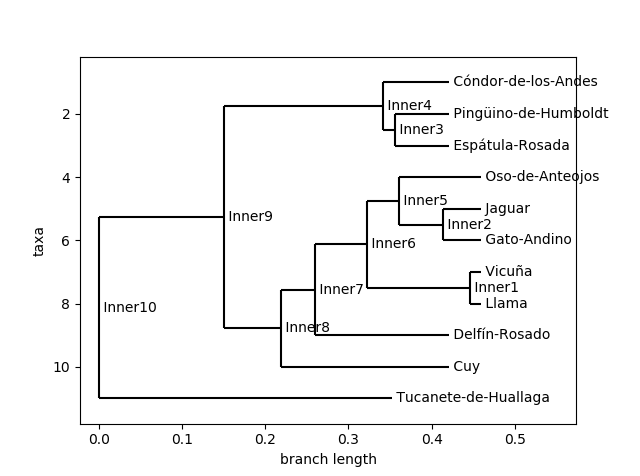
\includegraphics[width=12.5cm,height=8.5cm]{arbol.png}
	
	Fig. Arbol utilizando el metodo UPGMA
\end{center}

\subsection{Analizar el árbol filogenético}
Apartir del arbol filogenetico se podra descubrir/Mostrar/Analizar las relaciones evoluticas de las especies endemicas escogidas.
\subsubsection{Modelamiento de la Estrutura de Proteinas}
En el analisis se encuentra el modelamiento de la Estructura de Proteinas

\section{Conclusiones}
Incluye las ventajas y desventajas del enfoque utilizado, aspectos inesperados del proyecto, trabajo futuro, etc.
\section{Apéndice}


\end{document}